\documentclass[twocolumn, 10pt, letterpaper]{article}

% Font
\usepackage[utf8]{inputenc}
\usepackage{MinionPro} 
\input{glyphtounicode}
\pdfgentounicode=1 
\usepackage{microtype}

% Format
\usepackage[letterpaper, margin = 1in]{geometry}
\setcounter{secnumdepth}{0}
\usepackage{authblk}
% \renewcommand\Affilfont{\small}
% \usepackage[hang, flushmargin]{footmisc}
\setlength{\columnsep}{15pt}

% Links
\usepackage[colorlinks = true, linkcolor = black, urlcolor = black, citecolor = black]{hyperref} 

% Figures
\usepackage{graphicx}
\usepackage[labelfont = bf, labelsep = newline, singlelinecheck = false]{caption}

% Tables
\usepackage{booktabs}
\usepackage{tabularx}
\usepackage[table, xcdraw]{xcolor}

\begin{document}

(Pettigrew \& Tropp, 2006)

\hypertarget{results}{%
\section{Results}\label{results}}

\hypertarget{search-results}{%
\subsection{Search results}\label{search-results}}

\begin{figure*}[!t]
\centering
\caption{Flow diagram illustrating the preregistered search strategy, study selection, and data collection}
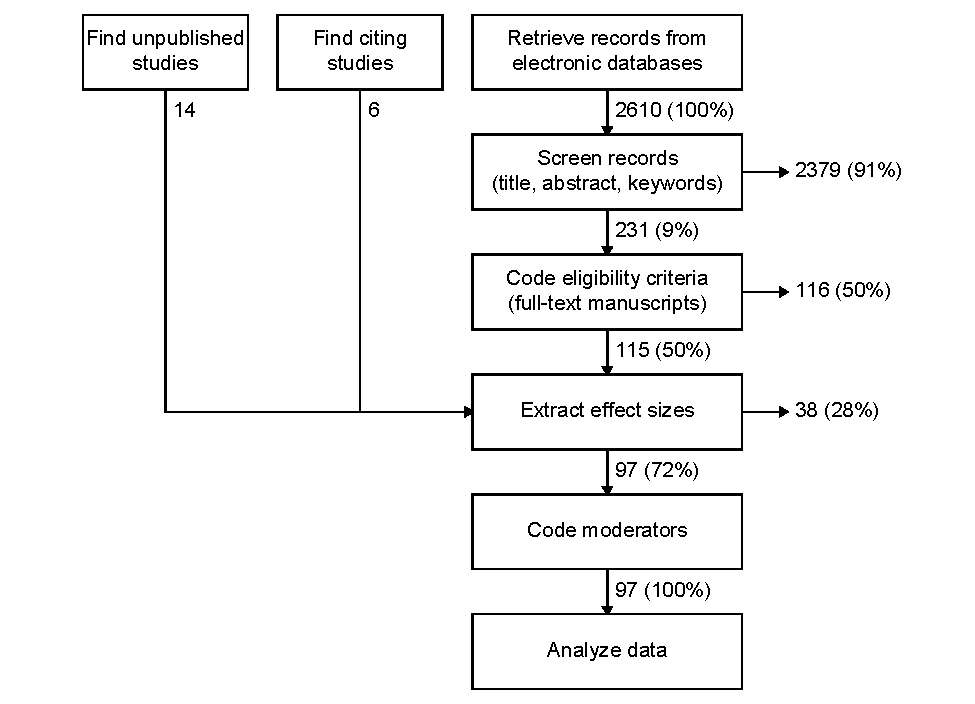
\includegraphics[scale=1]{../figures/figure-1}
\label{fig:f1}
\end{figure*}

\begin{figure*}
\centering
\caption{Overview of the relevant literature}
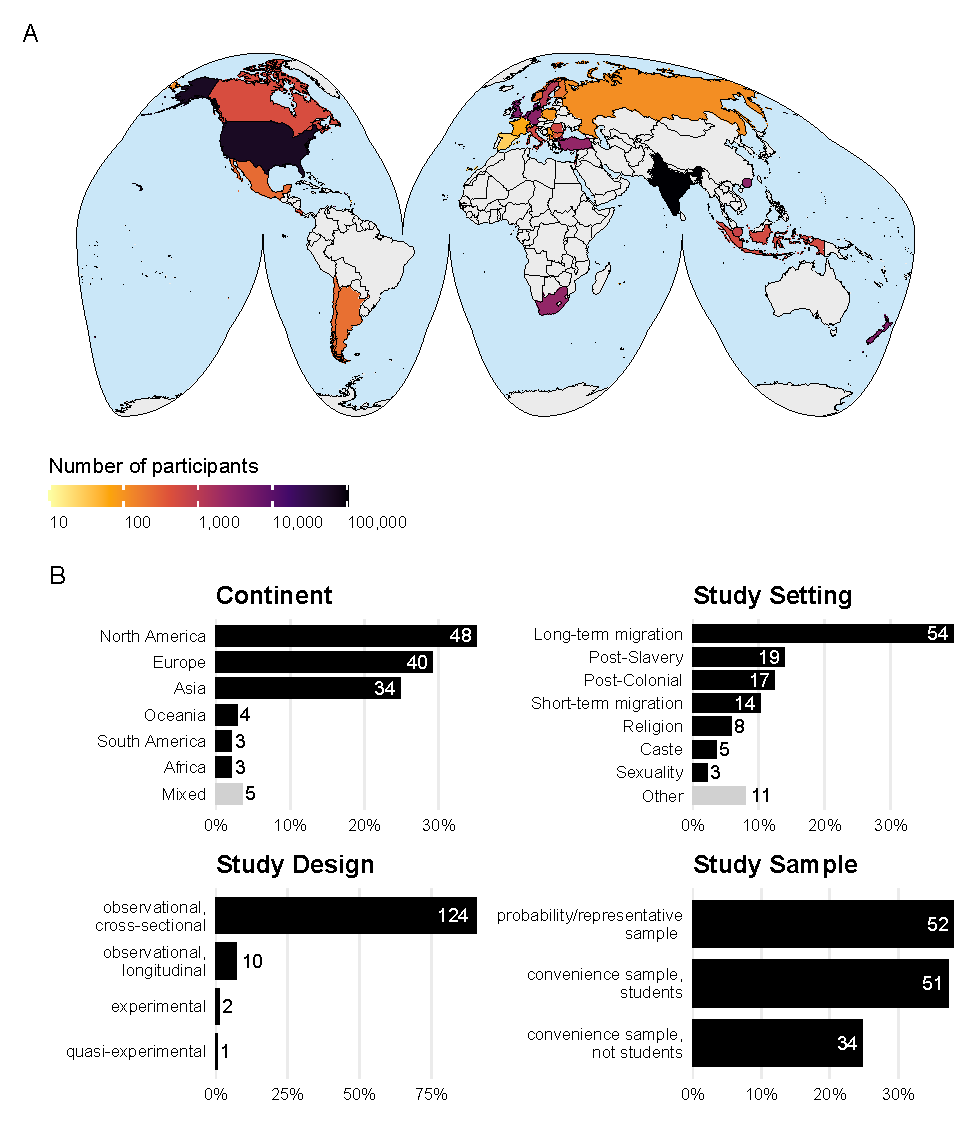
\includegraphics[scale=1]{../figures/figure-2}
\caption*{\textit{Note.} \textbf{A} Map of all countries included in the meta-analysis with combined sample sizes. \textbf{B} Proportion of eligible samples in each category as well as the absolute number of samples in each category.}
\label{fig:f2}
\end{figure*}

\hypertarget{preregistered-analyses}{%
\subsection{Preregistered analyses}\label{preregistered-analyses}}

As preregistered, we ran three random-effects meta-analysis models, one
for each outcome variable. Figure 3 shows posterior distributions from
these analyses.

\begin{figure*}
\centering
\caption{Posterior distributions from the preregistered random-effect meta-analysis models}
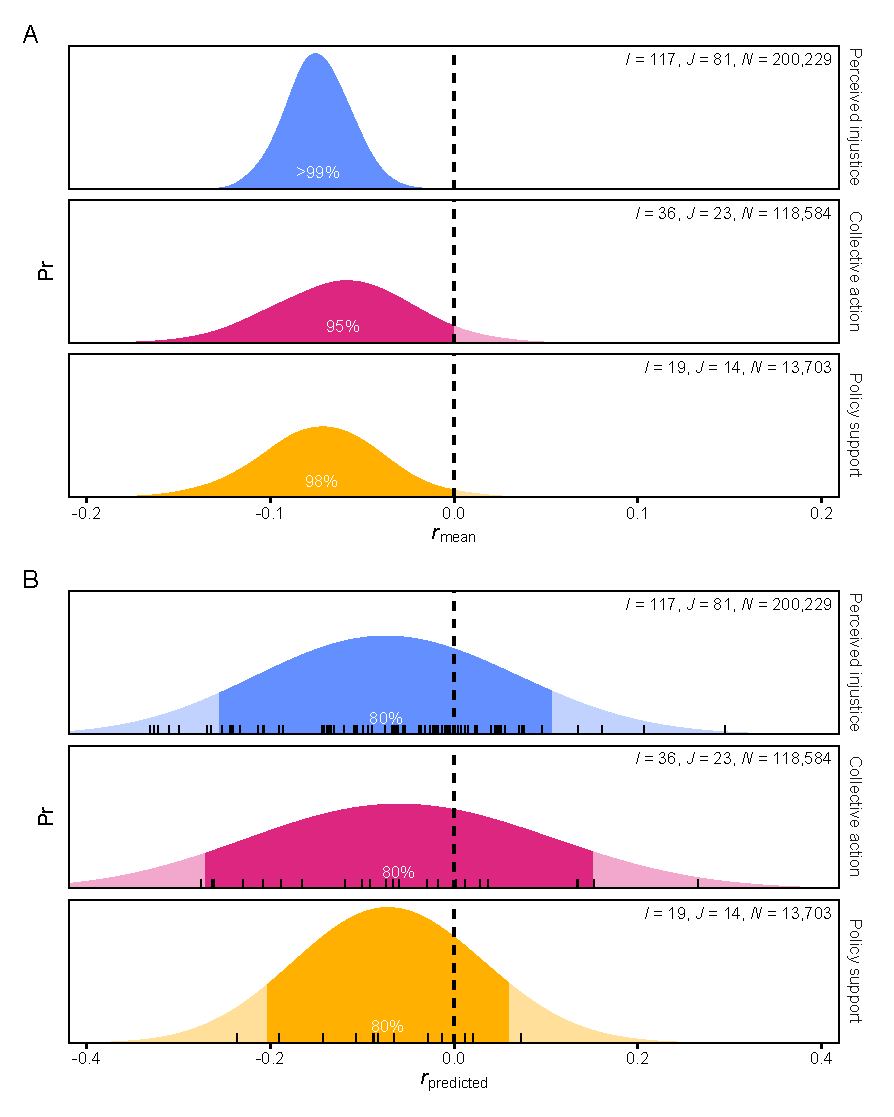
\includegraphics[scale=1]{../figures/figure-3}
\caption*{\textit{Note.} \textbf{A} Posterior distributions for the estimated mean correlation coefficients, highlighting the proportion of posterior samples for which $r_\text{mean} < 0$. \textbf{B} Posterior predictive distributions for the estimated study-wise correlation coefficients, based on point estimates of the $\mu$ and $\tau_J$ parameters, with point estimates for the estimated correlation coefficients for all studies in the sample.}
\label{fig:f3}
\end{figure*}

\emph{Perceived injustice.} Across 201,912 participants from 123 samples
in 84 studies, we found strong evidence for a weak association
(\(r = -.07, [-.10, -.04]\)) between intergroup contact and perceived
injustice, with \(>99.9\%\) of posterior samples for the mean
correlation coefficient falling below zero. We found evidence that
correlation coefficients varied across studies
(\(\tau_J = .14, [.12, .17]\)) and across samples within studies
(\(\tau_I = .08, [.05, .12]\)). Based on these analyses, we predicted
that 80\% of studies would result in correlation coefficients between
-.25 and .11 and that researchers would need sample sizes of at least
2,538 participants to find significant associations (\(\alpha = .05\),
two-sided) in 80\% of their studies.\footnote{Sample sizes are based on
  posterior predictions from the three models, which implied that, for
  80\% of studies, the absolute correlation coefficient would be
  \(|r| > .039\) for perceived injustice, \(|r| > .045\) for collective
  action, and \(|r| > .035\) for policy support.}

\emph{Collective action.} Across 119,085 participants from 37 samples in
24 studies, we found some evidence for a weak association
(\(r = -.06, [-.13, .02]\)) between intergroup contact and collective
action, with \(93.6\%\) of posterior samples for the mean correlation
coefficient falling below zero. We found evidence that correlation
coefficients varied across studies (\(\tau_J = .16, [.12, .23]\)) and
across samples within studies (\(\tau_I = .09, [.06, .14]\)). Based on
these analyses, we predicted that 80\% of studies would result in
correlation coefficients between -.27 and .16 and that researchers would
need sample sizes of at least 1,882 participants to find significant
associations (\(\alpha = .05\), two-sided) in 80\% of their studies.

\emph{Policy support.} Across 13,703 participants from 19 samples in 14
studies, we found some evidence for a weak association
(\(r = -.07, [-.14, -.00]\)) between intergroup contact and policy
support, with \(98.1\%\) of posterior samples for the mean correlation
coefficient falling below zero. We found evidence that correlation
coefficients varied across studies (\(\tau_J = .10, [.06, .18]\)) and,
to a lesser extent, across samples within studies
(\(\tau_I = .03, [.00, .12]\)). Based on these analyses, we predicted
that 80\% of studies would result in correlation coefficients between
-.21 and .07 and that researchers would need sample sizes of at least
3,208 participants to find significant associations (\(\alpha = .05\),
two-sided) in 80\% of their studies.

As preregistered, we ran another three random-effects meta-analysis
models to estimate the relationships between the three outcome
variables. As we were not interested in the direction of these
relationships, we used cross-sectional correlation coefficients as
effect sizes for longitudinal studies. Across 111,753 participants from
25 samples in 14 studies, we found evidence for a moderate association
(\(r = .31, [.23, .38]\)) between perceived injustice and collective
action. Across 6,244 participants from 12 samples in 9 studies, we found
evidence for a moderate association (\(r = .23, [.08, .35]\)) between
perceived injustice and policy support. Across 8,558 participants from 6
samples in 3 studies, we found evidence for a moderate association
(\(r = .30, [.13, .42]\)) between collective action and policy support.

\hypertarget{robustness-checks}{%
\subsubsection{Robustness checks}\label{robustness-checks}}

First, we assessed to what extent our findings were sensitive to
choosing narrower, \(\mu \sim \text{Normal}(0, 0.1)\), or wider,
\(\mu \sim \text{Normal}(0, 1)\), prior distributions. Choosing narrower
or wider prior distribution did not affect mean effect size estimates
for perceived injustice (\(\Delta r = -.00, [-.05, .04]\) and
\(\Delta r = .00, [-.05, .05]\)), collective action
(\(\Delta r = -.01, [-.11, .09]\) and \(\Delta r = -.00, [-.10, .11]\)),
and policy support (\(\Delta r = -.01, [-.10, .08]\) and
\(\Delta r = .00, [-.09, .10]\)). Second, we assessed to what extent our
findings were sensitive to including or excluding influential studies by
repeating the preregistered analyses \(J\) times while leaving out one
of \(J\) studies each time and by calculating the mean absolute
difference (\emph{MAD}) for the estimated mean effect size across
left-out studies. For perceived injustice
(\(\textit{MAD} = .02, [.01, .04]\)), collective action
(\(\textit{MAD} = .04, [.02, .09]\)), and policy support
(\(\textit{MAD} = .03, [.02, .08]\)), the \emph{MAD} was small. Leaving
out the most influential study, for example, did not change estimates of
the mean effect size for the three outcomes
(\(\Delta r = .00, [-.04, .05]\); \(\Delta r = .02, [-.09, .12]\);
\(\Delta r = -.02, [-.11, .07]\)). Together, these analyses showed that
our findings were robust to choosing different prior distributions and
to excluding influential studies.

\hypertarget{references}{%
\section{References}\label{references}}

\begingroup

\noindent \setlength{\parindent}{-0.5in} \setlength{\leftskip}{0.5in}

\hypertarget{refs}{}
\leavevmode\hypertarget{ref-pettigrew_meta-analytic_2006}{}%
Pettigrew, T. F., \& Tropp, L. R. (2006). A meta-analytic test of
intergroup contact theory. \emph{Journal of Personality and Social
Psychology}, \emph{90}(5), 751--783.
\url{https://doi.org/10.1037/0022-3514.90.5.751}

\endgroup

\end{document}